% Created 2017-01-08 Sun 16:28
% Intended LaTeX compiler: pdflatex
\documentclass[presentation,smaller]{beamer}
\RequirePackage{etex}
\RequirePackage[l2tabu,orthodox]{nag}            %% Warn about obsolete commands and packages
\RequirePackage{amsmath,amsfonts,amssymb,amsthm} %% Math
\RequirePackage{ifxetex,ifluatex}                %% Detect XeTeX and LuaTeX
\RequirePackage{fixltx2e}                        %% provides \textsubscript
\RequirePackage{xspace}
\RequirePackage{graphicx}
\RequirePackage{comment}
\RequirePackage{url}
\RequirePackage{relsize}
\RequirePackage{booktabs}
\RequirePackage{tabularx}
\RequirePackage[normalem]{ulem}
\RequirePackage[all]{xy}

%%%
%%% Code Listings
%%%

\RequirePackage{listings}
\lstdefinelanguage{Sage}[]{Python}{morekeywords={True,False,sage,cdef,cpdef,ctypedef,self},sensitive=true}

\lstset{frame=none,
  showtabs=False,
  showspaces=False,
  showstringspaces=False,
  commentstyle={\color{gray}},
  keywordstyle={\color{mLightBrown}\textbf},
  stringstyle ={\color{mDarkBrown}},
  frame=single,
  basicstyle=\tt\scriptsize\relax,
  backgroundcolor=\color{gray!190!black},
  inputencoding=utf8,
  literate={…}{{\ldots}}1,
  belowskip=0.0em,
}

%%%
%%% Tikz
%%%

\RequirePackage{tikz,pgfplots}

\usetikzlibrary{calc}
\usetikzlibrary{arrows}
\usetikzlibrary{automata}
\usetikzlibrary{positioning}
\usetikzlibrary{decorations.pathmorphing}
\usetikzlibrary{backgrounds}
\usetikzlibrary{fit,}
\usetikzlibrary{shapes.symbols}
\usetikzlibrary{chains}
\usetikzlibrary{shapes.geometric}
\usetikzlibrary{shapes.arrows}
\usetikzlibrary{graphs}

%% Cache

\ifdefined\tikzcaching  % chktex 1
  \usetikzlibrary{external}
  \tikzexternalize[prefix=build/]
  \tikzset{external/up to date check=diff}  %% MD5 fails from within emacs
\fi

%%%
%%% SVG (Inkscape)
%%%

\ifxetex % chktex 1
\newcommand{\executeiffilenewer}[3]{%
  {\immediate\write18{#3}} % hack
}
\else
\newcommand{\executeiffilenewer}[3]{%
  \ifnum\pdfstrcmp{\pdffilemoddate{#1}}%
    {\pdffilemoddate{#2}}>0%
    {\immediate\write18{#3}}
  \fi%
}
\fi

\newcommand{\includesvg}[2][1.0\textwidth]{%
 \executeiffilenewer{#1.svg}{#1.pdf}%
 {inkscape -z -D --file=#2.svg --export-pdf=#2.pdf --export-latex --export-area-page}%
 \def\svgwidth{#1} 
 \input{#2.pdf_tex}%
} 

%%%
%%% Metropolis Theme
%%%

\usetheme{metropolis}
\metroset{color/block=fill}
\metroset{numbering=none}
\metroset{outer/progressbar=foot}
\metroset{titleformat=smallcaps}

\setbeamercolor{description item}{fg=mLightBrown}
% \setbeamerfont{alerted text}{series=\bfseries}
\setbeamerfont{footnote}{size=\scriptsize}
\setbeamercolor{example text}{fg=mDarkBrown}

\renewcommand*{\UrlFont}{\ttfamily\smaller\relax}

%%%
%%% UTF-8
%%% 

\RequirePackage{unicodesymbols} % after metropolis which loads fontspec

%%%
%%% BibLaTeX
%%%

\RequirePackage[backend=bibtex,
            style=alphabetic,
            maxnames=4,
            citestyle=alphabetic]{biblatex}

\bibliography{local.bib,abbrev3.bib,crypto_crossref.bib,rfc.bib,jacm.bib}

\DeclareFieldFormat{title}{\alert{#1}}
\DeclareFieldFormat[book]{title}{\alert{#1}}
\DeclareFieldFormat[thesis]{title}{\alert{#1}}
\DeclareFieldFormat[inproceedings]{title}{\alert{#1}}
\DeclareFieldFormat[incollection]{title}{\alert{#1}}
\DeclareFieldFormat[article]{title}{\alert{#1}}
\DeclareFieldFormat[misc]{title}{\alert{#1}}

%%% 
%%% Microtype
%%%

\IfFileExists{upquote.sty}{\RequirePackage{upquote}}{}
\IfFileExists{microtype.sty}{\RequirePackage{microtype}}{}

\setlength{\parindent}{0pt}                   %%
\setlength{\parskip}{6pt plus 2pt minus 1pt}  %%
\setlength{\emergencystretch}{3em}            %% prevent overfull lines
\setcounter{secnumdepth}{0}                   %%

%%% Local Variables:
%%% mode: latex
%%% End:
\usepackage{graphicx}
\usepackage{grffile}
\usepackage{longtable}
\usepackage{wrapfig}
\usepackage{rotating}
\usepackage[normalem]{ulem}
\usepackage{amsmath}
\usepackage{textcomp}
\usepackage{amssymb}
\usepackage{capt-of}
\usepackage{hyperref}
\usepackage{microtype}
\usepackage{newunicodechar}
\usepackage{unicodesymbols}
\usepackage[notions,operators,sets,keys,ff,adversary,primitives,complexity,asymptotics,lambda,landau]{cryptocode}
\usepackage{xspace}
\usepackage{units}
\usepackage{nicefrac}
\usepackage{gensymb}
\usepackage{amsthm}
\usepackage{amsmath}
\usepackage{amssymb}
\usepackage{xcolor}
\usepackage{listings}
\usepackage[color=yellow!40]{todonotes}
\newcommand{\ZZ}[1][blank]{\ensuremath{\ifthenelse{\equal{#1}{blank}}{\mathbb{Z}}{\mathbb{Z}\left[#1\right]}\xspace}}
\usepackage{filecontents}
\usepackage{url}
\usefonttheme[onlymath]{serif}
\renewcommand{\vec}[1]{\ensuremath{\mathbf{#1}}\xspace}
\newcommand{\sample}{\ensuremath{\leftarrow_{\$}}}
\newcommand{\ovec}[1]{\ensuremath{\overline{\vec{#1}}}\xspace}
\setbeamercolor{example text}{fg=mDarkBrown}
\usetheme{default}
\author{Martin R. Albrecht \textbf{@martinralbrecht}}
\date{22/08/2016 — Big-O London}
\title{Greatest Common Divisors: Attacks on RSA and Post-Quantum Security}
\hypersetup{
pdfauthor={Martin R. Albrecht \textbf{@martinralbrecht}},
pdftitle={Greatest Common Divisors: Attacks on RSA and Post-Quantum Security},
pdfkeywords={},
pdfsubject={},
pdfcreator={Emacs 25.1.1 (Org mode 9.0.3)},
pdflang={English},
colorlinks,
citecolor=gray,
filecolor=gray,
linkcolor=gray,
urlcolor=gray
}
\begin{document}

\maketitle
\begin{frame}{Outline}
\tableofcontents
\end{frame}



\section{Greatest Common Divisors}
\label{sec:orge79265a}

\begin{frame}[fragile,label={sec:org82cccc9}]{Euclidean algorithm}
 Given two integers \(a, b < N = 2^κ\) the Euclidean algorithm computes their greatest common divisor \(\gcd(a,b)\).

\lstset{language=Python,label= ,caption= ,captionpos=b,numbers=none}
\begin{lstlisting}
def gcd(a, b):
    if b == 0:
        return a
    else:
        return gcd(b, a % b)
\end{lstlisting}

\begin{itemize}
\item The Euclidean algorithm runs in time \(\bigO{κ^2}\).
\item Best known algorithm runs in time \(\bigO{κ \log^2 κ \log\log κ}\). \footfullcite{ANTS:SteZim04}
\end{itemize}
\end{frame}

\section{RSA}
\label{sec:org888da86}

\begin{frame}[label={sec:org65b588d}]{Public key encryption}
\begin{description}
\item[{KeyGen}] Bob sends padlock \alert{\(pk\)} to Alice and keeps the key \alert{\(sk\)}.

\item[{Enc}] Alice inserts message \alert{\(m\)} in a box and locks it with \alert{\(pk\)}.

\item[{Dec}] Bob opens the box \alert{\(c\)} with key \alert{\(sk\)} to the padlock \alert{\(pk\)}.
\end{description}
\end{frame}

\begin{frame}[label={sec:orgd9276f5}]{Public key encryption}
\begin{description}
\item[{KeyGen}] Bob generates a key pair \alert{\((sk, pk)\)} and publishes \alert{\(pk\)}.

\item[{Enc}] Alice uses \alert{\(pk\)} to encrypt message \alert{\(m\)} for Bob as \alert{\(c\)}.

\item[{Dec}] Bob uses \alert{\(sk\)} to decrypt \alert{\(c\)} to recover \alert{\(m\)}.
\end{description}
\end{frame}

\begin{frame}[label={sec:org6023a3d}]{Naive RSA}
\begin{description}
\item[{KeyGen}] The public key is \((N,e)\) and the private key is \(d\), with

\begin{itemize}
\item \(N = p⋅q\) where \(p\) and \(q\) prime,
\item \(e\) coprime to \(φ(N) = (p-1)(q-1)\) and
\item \(d\) such that \(e⋅ d = 1 \mod{φ(N)}\).
\end{itemize}

\item[{Enc}] \(c = m^e \mod{N}\)

\item[{Dec}] \(m = c^d = m^{e\cdot d} = m^{1} \mod{N}\)
\end{description}
\end{frame}

\begin{frame}[label={sec:org5f0bde3}]{Naive RSA is not IND-CCA secure}
\begin{itemize}[<+->]
\item Assume we want to decrypt \(c = m^e \bmod N\) with access to an oracle which will decrypt any ciphertext but \(c\).

\item Pick a random \(s \bmod N\) and compute \(c' = s^e ⋅ c \bmod N\)

\item Submit \(c'\) to the decryption oracle to recover \(m' = {\left(s^e ⋅ c\right)}^d\)

\item It holds that

\[m' = {\left(s^e ⋅ c\right)}^d = {\left(s^e ⋅ m^e\right)}^d = {\left({\left(s⋅m\right)}^e \right)}^d = s⋅m \bmod N\]

\item Such an oracle can essentially be instantiated using error messages. \footfullcite{C:Bleichenbacher98}
\end{itemize}
\end{frame}

\begin{frame}[label={sec:orgdef03c8}]{RSA-OAEP}
\begin{center}
\begin{center}
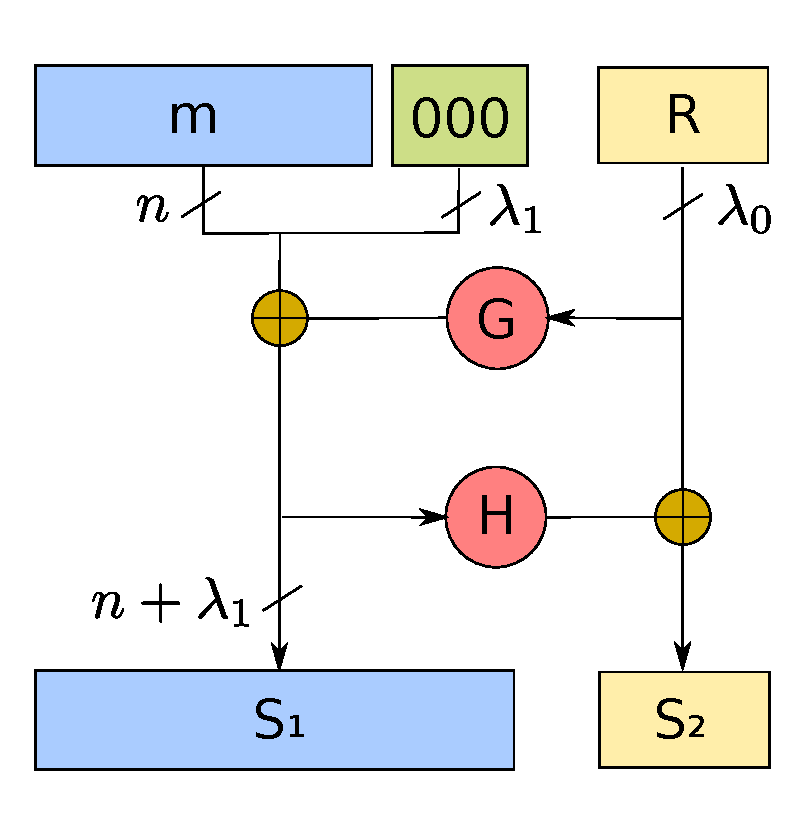
\includegraphics[width=0.5\textwidth]{./rsa-oaep.pdf}
\end{center}
\end{center}

Use RSA-OAEP (also sometimes called "PKCS\#1 v2.1 encryption").
\end{frame}

\begin{frame}[label={sec:orgea0b0c7}]{“We use RSA!”}
\begin{description}
\item[{boxcryptor}] \begin{center}
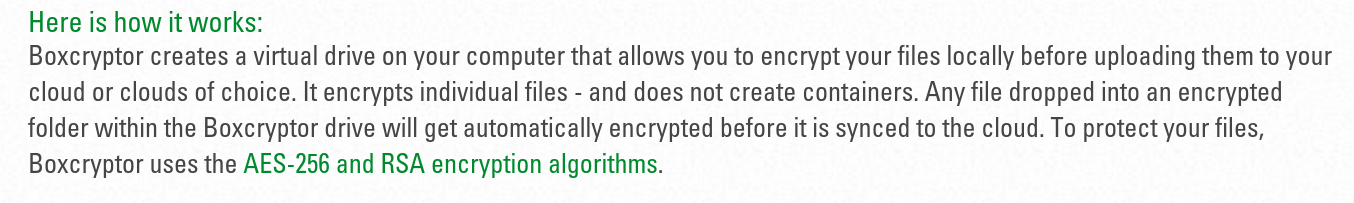
\includegraphics[width=.9\linewidth]{./boxcryptor.png}
\end{center}
\item[{telegram}] \begin{center}
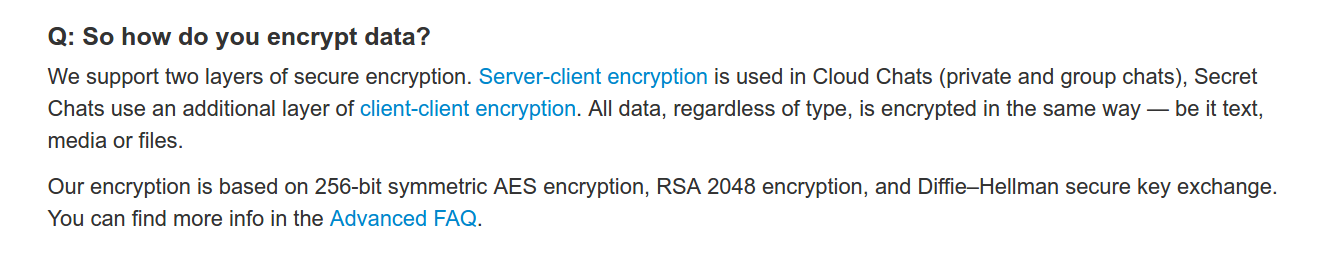
\includegraphics[width=.9\linewidth]{./telegram.png}
\end{center}
\item[{sicher}] \begin{center}

\includegraphics[width=.9\linewidth]{./sicher.png}
\end{center}
\end{description}
\end{frame}

\begin{frame}[label={sec:orge96d1e6}]{Classical attacks on RSA}
\begin{itemize}
\item An adversary who can factor large integers can break RSA.

\item The best known classical algorithm for factoring is the Number Field Sieve (NFS)

\item It has a \alert{super-polynomial} but \alert{sub-exponential} (in \(\log N\) ) complexity of \[\bigO{e^{1.9 (\log^{1/3} N) (\log\log^{2/3} N)}}\] operations.
\end{itemize}


\pause

\begin{block}{Warning}
This does not mean an adversary \textbf{has} to factor to solve RSA.
\end{block}
\end{frame}

\section{The GCD attack on bad random numbers}
\label{sec:org7703e79}
\begin{frame}[label={sec:org5ee5f72}]{Much randomness}
\begin{itemize}
\item When we generate RSA moduli, we need to sample two good prime numbers of bitsize \(κ/2\)
\item The probability that a random number of bitsize \(κ/2\) is prime, is about \(1/κ\).
\item To sample an RSA modulus we hence need about \(κ^2\) random bits. For \(κ = 1024\) this means about \(10^6\) random bits.
\item Where do we get all these bits from?
\end{itemize}
\end{frame}

\begin{frame}[label={sec:org19350d4}]{Collecting entropy}
Random bits can be gathered from the environment using various sensors, e.g.

\begin{itemize}
\item time,
\item process IDs currently running on the machine,
\item the harddisk,
\item the content of uninitialised memory,
\item hardware sensors (temperature etc.).
\end{itemize}
\end{frame}

\begin{frame}[label={sec:org2799b3f}]{What could possibly go wrong?}
Assume a router generating RSA moduli on booting for the first time.

\begin{itemize}
\item It might not know the time but retrieve it once booted.
\item Whenever it boots the same processes are running.
\item The harddisk has the same files on it for every router.
\item Uninitialised memory is just full of zeros.
\item There are perhaps no hardware sensors.
\end{itemize}

All routers of the same make might (in fact, some do) generate the \alert{same} RSA modulus.
\end{frame}

\begin{frame}[label={sec:orgaa09002}]{What could possibly go wrong?}
What if two routers generate moduli \(N_0 = q_0 ⋅ p\) and \(N_1 = q_1 \cdot p\), i.e. moduli with shared factors, due to bad randomness?

\begin{itemize}
\item We assume that factoring each of \(N_0\) or \(N_1\) is hard.
\item However, computing \(\gcd(N_0, N_1)\) reveals \(p\) but costs only \(\bigO{\log^2 N}\) operations.
\end{itemize}

\pause
If only we could compute the pairwise GCD of all RSA moduli on the Internet \dots{}
\end{frame}

\begin{frame}[label={sec:orgab72a6c}]{The GCD attack on poor random numbers}
\begin{quote}
[W]e are able to compute the private keys for 64,000 (0.50\%) of the TLS hosts and 108,000 (1.06\%) of the SSH hosts from our scan data alone by exploiting known weaknesses of RSA and DSA when used with insufficient randomness.\footfullcite{USENIX:HDWH12}
\end{quote}
\end{frame}

\begin{frame}[label={sec:orgb689215}]{Computing pairwise GCDs efficiently}
\begin{itemize}[<+->]
\item Naively, we’d have to compute \(\bigO{t^2}\) GCDs to check all \(t\) moduli against each other.
\item We can do better by performing \(t\) GCD computations \[\gcd(N_i, \prod_{j \neq i} N_j)\]
\item We will use the identity \[x \bmod N_0 = (x \bmod N_0⋅N_1) \bmod N_0\]
\end{itemize}
\end{frame}

\begin{frame}[label={sec:org11ba7d2}]{Computing pairwise GCDs efficiently}
Let, for example, \(t = 4\).

\begin{center}
\begin{tikzpicture}[node distance=3cm,on grid,scale=0.6, every node/.style={transform shape}]
\node[anchor=center] (N0) at (0,0) {$N_0$};
\node[anchor=center] (N1) at (4,0)  {$N_1$};
\node[anchor=center] (N2) at (8,0) {$N_2$};
\node[anchor=center] (N3) at (12,0) {$N_3$};

\node[anchor=center](N01) at (2, -2) {$N_{01} = N_{0}\cdot N_1$};
\node[anchor=center] at (10, -2) (N23) {$N_{23} = N_{2} \cdot N_3$};

\node[anchor=center](N0123) at (6,-4) {$N_{0123} = N_{01} \cdot N_{23}$};

\draw (N0) -- (N01);
\draw (N1) -- (N01);

\draw (N2) -- (N23);
\draw (N3) -- (N23);

\draw (N01) -- (N0123);
\draw (N23) -- (N0123);

\node[] (M01) at (2,-6) {$M_{01} = N_{0123} \bmod N_{01}^2$};
\node[] (M23) at (10,-6)  {$M_{23} = N_{0123} \bmod N_{23}^2$};

\node[] (M0) at (-1,-8)  {$M_{0} = M_{01} \bmod N_{0}^2$};
\node[] (M1) at (4,-8) {$M_{1} = M_{01} \bmod N_{1}^2$};

\node[] (M2) at (8,-8) {$M_{2} = M_{23} \bmod N_{2}^2$};
\node[] (M3) at (12,-8) {$M_{3} = M_{23} \bmod N_{3}^2$};

\draw (N0123) -- (M01);
\draw (N0123) -- (M23);

\draw (M01) -- (M0);
\draw (M01) -- (M1);
\draw (M23) -- (M2);
\draw (M23) -- (M3);

\end{tikzpicture}
\end{center}

\begin{itemize}
\item Compute \(R_{1} = \gcd(M_{1}/N_{1}, N_1), \dots, R_{4} = \gcd(M_{4}/N_{4}, N_{4})\)
\item Cost: \(\bigO{t ⋅ κ ⋅ \log^2 (t ⋅ κ) \log\log (t ⋅ κ)}\)
\end{itemize}
\end{frame}

\section{The Approximate GCD problem}
\label{sec:org05860d6}
\begin{frame}[label={sec:orgb9dc13f}]{Quantum attacks on RSA}
An adversary with access to a quantum computer with \[ \bigO{\log^2(N) \log\log (N) \log\log\log (N)}\] gates can factor \(N\) using Shor’s algorithm.\footnote{\url{http://www.scottaaronson.com/blog/?p=208}}
\end{frame}

\begin{frame}[label={sec:org93a2aef}]{Quantum attacks on RSA}
\begin{center}
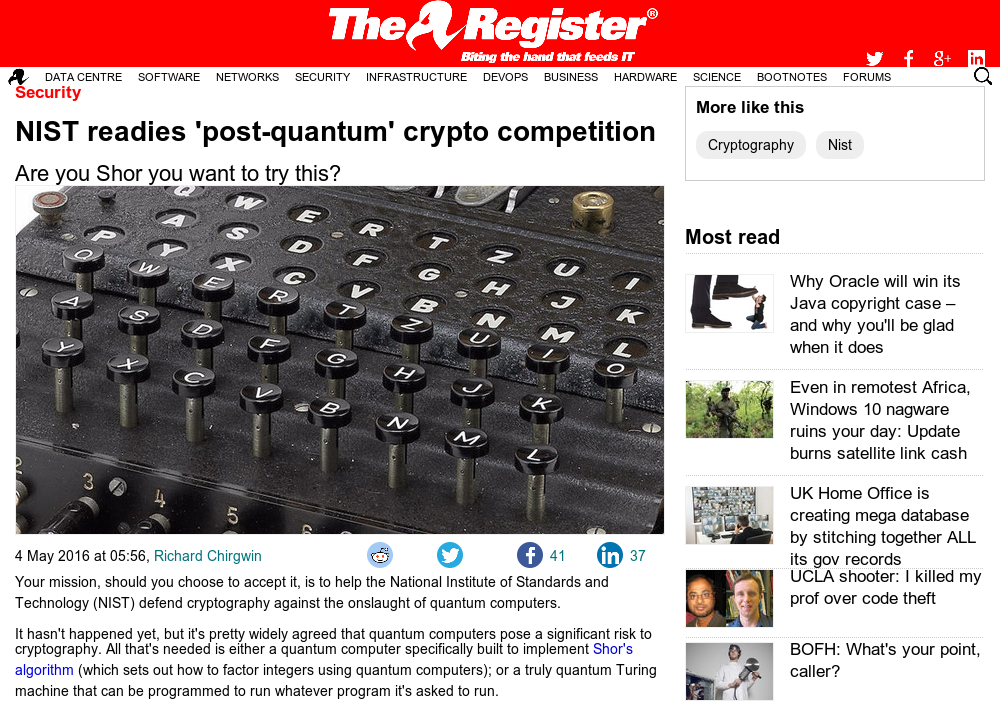
\includegraphics[width=.9\linewidth]{./competition.png}
\end{center}
\end{frame}

\begin{frame}[label={sec:org2ceec0e}]{The Approximate GCD problem}
The \alert{Approximate GCD} problem is the problem of distinguishing \[x_i = q_i ⋅ p  \alert{+ r_i}\] from uniform \(\ZZ ∩ [0, X)\) with \(x_i < X\).
\end{frame}

\begin{frame}[label={sec:org0c4ebc0}]{The Approximate GCD problem}
\[x_i = q_i ⋅ p  + r_i\]

If \(λ\) is our security parameter (think \(λ=128\)), then

\begin{center}
\begin{tabular}{rrll}
name & sizeof & DGHV10 \footfullcite{EC:DGHV10} & CheSte15 \footfullcite{EC:CheSte15}\\
\hline
\(γ\) & \(x_i\) & \(λ^5\) & \(λ \log λ\)\\
\(η\) & \(p\) & \(λ^2\) & \(λ + \log λ\)\\
\(ρ\) & \(r_i\) & \(λ\) & \(λ\)\\
\end{tabular}

\end{center}
\end{frame}

\begin{frame}[label={sec:org5350706}]{Naive encryption}
\begin{description}
\item[{KeyGen}] The public key is \(\{x_i = q_i ⋅ p + 2\,r_i\}_{0 ≤ i < t}\) and the private key is \(p\).

\item[{Enc}] For \(m \in \{0,1\}\) output \(c = m + \sum b_i ⋅ x_i\) with \(b_i \sample \{0,1\}\).

\item[{Dec}] \(m = (c \bmod p) \bmod 2\).
\end{description}

\pause

\begin{block}{Warning}
This encryption scheme has the same malleability property as naive RSA encryption!\footnote{In contrast to naive RSA, this scheme offers indistinguishability security under chosen plaintext attacks (IND-CPA).}
\end{block}
\end{frame}

\section{Attacks on the Approximate GCD problem}
\label{sec:org6fb52bc}

\begin{frame}[label={sec:orgd333adb}]{Exhaustive search}
Given \(x_0 = q_0 ⋅ p + r_0\) and \(x_1 + q_1 ⋅ p + r_1\) we know that \[p = \gcd\left((x_0 - r_0), (x_1 - r_1)\right)\]


Guess \(r_0\) and \(r_1\)!

\begin{block}{Cost}
\(2^{2ρ}\) GCDs
\end{block}
\end{frame}

\begin{frame}[label={sec:org100f612}]{Exhaustive search + multiplication}
Compute \[\gcd\left(x_0', \prod_{i=0}^{2^ρ-1} (x_1 - i) \bmod x_0'\right)\] for all \(x_0' = x_0 - j\) with \(0 \leq j < 2^{ρ-1}\).

\begin{block}{Cost}
\(2^ρ\) GCDs, \(2^{2ρ}\) multiplications
\end{block}
\end{frame}

\begin{frame}[label={sec:org55da4cd}]{Time-memory trade-off}
\begin{itemize}
\item We can reduce multiplications to \(2^{ρ/2}\) per guess of \(x_0'\).
\item Define univariate polynomials mod \(x_0'\):
\end{itemize}
\[f_j(x) = \prod_{i=0}^{j-1} (x_1 - (x + i)) \in \ZZ_{x_0'}[x]\]
\begin{itemize}
\item Note that
\end{itemize}
\[\prod_{i=0}^{2^ρ-1} (x_1 - i) = \prod_{k=0}^{2^{ρ/2} -1} f_{2^{ρ/2}}(2^{ρ/2}k)\]

\begin{block}{Example}
\begin{itemize}
\item \(ρ = 2\), \(f_{2} = (x_1 - (x + 0)) \cdot (x_1 - (x + 1))\)
\item \(f_{2}(0) ⋅ f_{2}(2) = (x_1 - 0) ⋅ (x_1 - 1) ⋅ (x_1 - 2) ⋅ (x_1 - 3)\)
\end{itemize}
\end{block}
\end{frame}

\begin{frame}[label={sec:orgc912992}]{Time-memory trade-off}
Compute \[\gcd\left(x_0', \prod_{k=0}^{2^{ρ/2} -1} f_{2^{ρ/2}}(2^{ρ/2}k) \bmod x_0'\right)\] for all \(x_0' = x_0 - j\) with \(0 \leq j < 2^{ρ-1}\).

\begin{block}{Cost}
\begin{itemize}
\item \(2^{ρ}\) GCDs and computation of \(f_{2^{ρ/2}}(x) \bmod x_0'\),
\item per guess for \(x_0'\): \(2^{ρ/2}\) multiplications and evaluations of \(f_{2^{ρ/2}}(x)\).
\end{itemize}
\end{block}
\end{frame}

\begin{frame}[label={sec:org316e7b2}]{Time-memory trade-off}
\begin{itemize}
\item Computing \(f_{2^{ρ/2}}(x) \bmod x_0'\) can be accomplished in time \(\bigO{2^{ρ/2} ⋅ ρ}\) using the Fast Fourier Transform.
\item Evaluating \(f_{2^{ρ/2}}(x) \bmod x_0'\) at our \(2^{ρ/2}\) points can be accomplished in time \(\bigO{2^{ρ/2} ⋅ ρ}\) using the Fast Fourier Transform.
\item The strategy is similar to the pairwise GCD case earlier
\end{itemize}

\begin{block}{Cost}
\(2^{\bigO{3/2 ρ \log^2 ρ}}\) operations.\footfullcite{EC:CheNgu12}
\end{block}
\end{frame}

\begin{frame}[label={sec:orga1e4b65}]{Lattice attacks}
Given \(x_0  = q_0 p + r_0\) and \(x_1  = q_1 p + r_1\), consider

\begin{eqnarray*}
q_0 x_1 - q_1 x_0 & = & q_0 (q_1 p + r_1) - q_1 (q_0 p - r_0)\\
                  & = & q_0 q_1 p + q_0 r_1 - q_1 q_0 p - q_1 r_0\\
& = & q_0 r_1 - q_1 r_0
\end{eqnarray*}

and note that \[q_0 x_1 - q_1 x_0 \ll x_i\]

\pause

\begin{block}{Non-starter?}
We don’t know \(q_i\)!
\end{block}
\end{frame}

\begin{frame}[label={sec:org267464b}]{Lattice attacks}
Consider the matrix 

\[\vec{B} = \begin{pmatrix}
2^{\rho + 1}  & x_1  & x_2   & \cdots  & x_t\\
              & -x_0 &       &         & \\
              &      &  -x_0 &         & \\
              &      &       &  \ddots & \\
              &      &       &         &  -x_0\\
\end{pmatrix}\]

multiplying on the left by the vector \(\vec{q} = (q_0, q_1, q_2, \cdots, q_t)\) gives
\begin{align*}
\vec{v} &= (q_0, q_1, \cdots, q_t) \cdot \vec{B} \\
        &= (q_0\, 2^{ρ+1}, q_0 x_1 - q_1 x_0, \cdots, q_0 x_t - q_t x_0)\\
        &= (q_0\, \alert{2^{ρ+1}}, q_0 \alert{r_1} - q_1 \alert{r_0}, \cdots, q_0 \alert{r_t} - q_t \alert{r_0})
\end{align*}
which is a vector with small coefficients compared to \(x_i\).
\end{frame}

\begin{frame}[label={sec:org4282223}]{Finding short vectors}
We call the set of all integer-linear combinations of the rows of \(\vec{B}\) the \alert{lattice} spanned by (the rows of) \(\vec{B}\).

\begin{description}
\item[{SVP}] finding a \alert{shortest} non-zero vector on \alert{general} lattices is NP-hard.

\item[{Gap-SVP}] finding \alert{short} non-zero vectors on \alert{general} lattices is a well-known and presumed quantum-hard problem.
\end{description}

\begin{block}{Easy SVP}
GCD is SVP on the integer lattice \(\ZZ\). For example, \(\vec{B} = {[21, 14]}^T\), \(\vec{v} = (-1,1)\), \(\vec{v} ⋅\vec{B} = 7\).
\end{block}
\end{frame}

\begin{frame}[label={sec:org6140301}]{Reduction to lattice problem}
We can show that an adversary \alert{has} to solve Gap-SVP.

\begin{block}{AGCD → LWE}
If there is an algorithm efficiently solving the AGCD problem then there exists an algorithm which solves the \textbf{Learning with Errors} (LWE) problem with essentially the same performance. \footfullcite{EC:CheSte15} 
\end{block}

\begin{block}{LWE → Gap-SVP}
If there is an algorithm efficiently solving the LWE problem then there exists a quantum algorithm which solves worst-case Gap-SVP instances.\footfullcite{STOC:Regev05}
\end{block}
\end{frame}

\section{Google’s post-quantum experiment: “A New Hope”}
\label{sec:org2ebc790}

\begin{frame}[label={sec:orga9a2bbc}]{Ring-LWE}
\begin{itemize}
\item The Learning with Errors problem is essentially the problem of solving a linear system of equations in the presence of noise.
\item Given \(\vec{A}, \vec{c}\) solve \[\vec{c} = \vec{A} ⋅ \vec{s} + \vec{e} \bmod q\] for \(\vec{s}\) when \(\vec{e}\) is “small”.
\item The matrix \(\vec{A} \in \ZZ_q^{m \times n}\) is kinda big.
\item To make it smaller, use \alert{structured matrices}, e.g. negacyclic matrices ⇒ Ring-LWE.
\end{itemize}
\end{frame}

\begin{frame}[fragile,label={sec:org922b6c1}]{A New Hope \footfullcite{EPRINT:ADPS15} : Ring-LWE based key exchange}
 \lstset{language=plantuml,label= ,caption= ,captionpos=b,numbers=none}
\begin{lstlisting}
skinparam monochrome true
skinparam dpi 600
skinparam backgroundColor transparent
skinparam classBackgroundColor transparent
skinparam style strictuml
skinparam handwritten true
skinparam packageStyle rect
skinparam defaultFontName FG Virgil

activate Client
Client -> Server: g<sup>a</sup>
activate Server
Client <- Server: g<sup>b</sup>, sign<sub>sk</sub>(g<sup>b</sup>)
note left: K= g<sup>ab</sup>
Client -> Server: E<sub>K</sub>(data)
note right: K= g<sup>ab</sup>
Server --> Client: E<sub>K</sub>(more data)
deactivate Server
deactivate Client
\end{lstlisting}

\begin{center}
\begin{center}
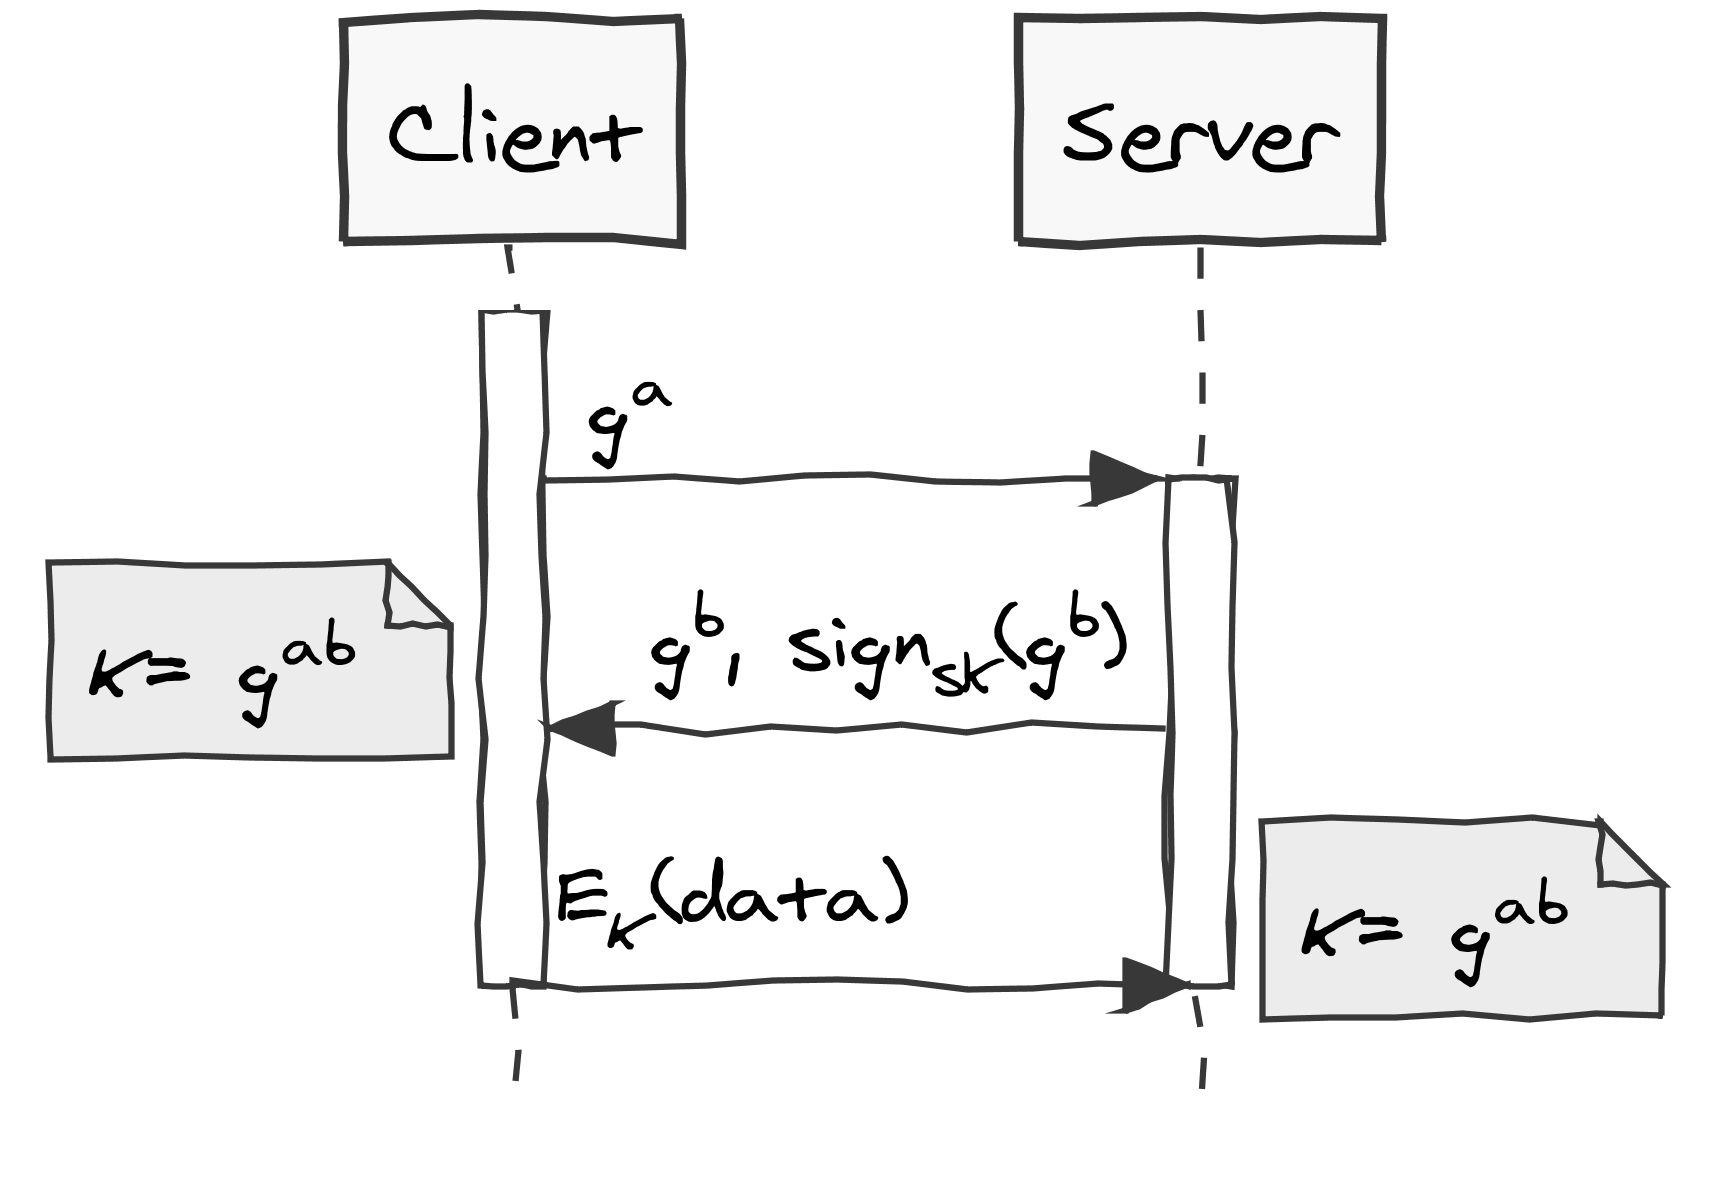
\includegraphics[width=0.6\textwidth]{keyex.png}
\end{center}
\end{center}
\end{frame}

\begin{frame}[label={sec:orgb7eee94}]{Thank you}
\begin{center}
\begin{center}
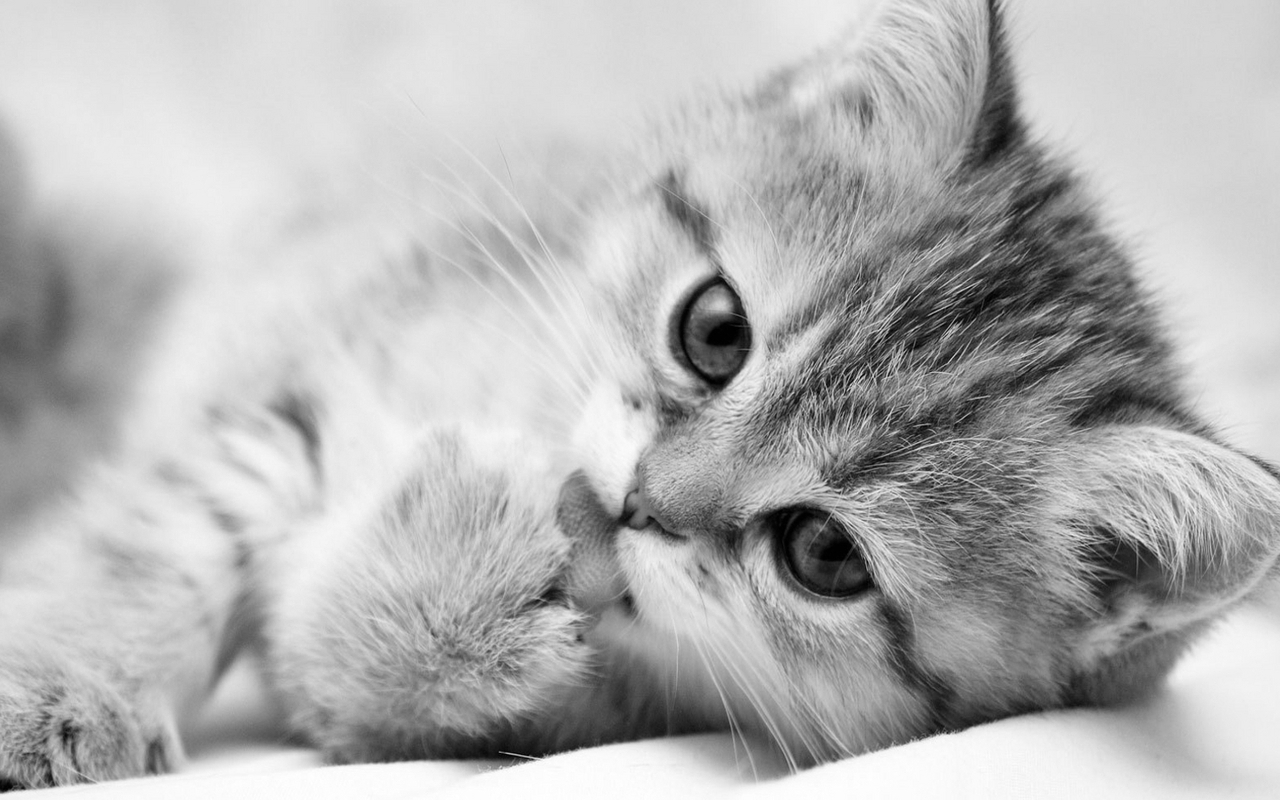
\includegraphics[width=.9\linewidth]{./kitten-01.jpg}
\end{center}

\alert{\Large Questions?}
\end{center}
\end{frame}

\section{Bonus}
\label{sec:org0cd8465}

\begin{frame}[label={sec:orgc1dbe83}]{Homomorphic encryption}
Given \(c_i = q_i ⋅ p + m_i'\) with \(m_i' = 2\,r_i + m_i\).
\begin{itemize}
\item We can compute \[c' = c_0 ⋅ c_1 = q_0 q_1 p^2 + q_0 m_1' p  + q_1 m_0' p + m_0' ⋅ m_1'\] to get \(c' \bmod p =  m_0' ⋅ m_1'\) and \(m_0' ⋅ m_1' \bmod 2 = m_0 ⋅ m_1\).
\item We can also compute \[c' = c_0 + c_1 = (q_0 + q_1) p + (m_0' + m_1')\] to get \(c' \bmod p \bmod 2 = m_0 \oplus m_1\).
\end{itemize}

We can compute with encrypted data.\footnote{\url{https://crypto.stanford.edu/craig/easy-fhe.pdf}}
\end{frame}
\end{document}